\documentclass[journal]{IEEEtran}

\usepackage{amsmath,amssymb,amsfonts,amsthm}
\usepackage{algorithmic}
\usepackage{graphicx}
\usepackage{textcomp}
\usepackage{xcolor}
\usepackage{booktabs}
\usepackage{cite}
\usepackage{url}
\usepackage{listings}
\usepackage{microtype}
\usepackage{hyperref}

\hypersetup{
    colorlinks=true,
    linkcolor=black,
    citecolor=black,
    urlcolor=blue
}

\newtheorem{theorem}{Theorem}
\newtheorem{definition}{Definition}

\lstset{
  language=R,
  basicstyle=\ttfamily\scriptsize,
  keywordstyle=\color{blue}\bfseries,
  commentstyle=\color{gray}\itshape,
  stringstyle=\color{teal},
  breaklines=true,
  breakatwhitespace=true,
  showstringspaces=false,
  numbers=left,
  numberstyle=\tiny\color{gray},
  frame=single,
  captionpos=b,
  tabsize=2
}

\begin{document}

\title{Distribution-Free Uncertainty Quantification in Machine Learning: A Theoretical and Empirical Comparison of Conformal Prediction, Bayesian Credible Intervals, and Parametric Bootstrap in R}

\author{Yuvraj~Chandak\quad and\quad Dr.~Veeramani~S%
\thanks{Yuvraj Chandak (Register No.: 25BCE2561) is with the School of Computer Science and Engineering, Vellore Institute of Technology, Vellore, Tamil Nadu 632014, India (e-mail: \href{mailto:yuvraj.chandak2025@vitstudent.ac.in}{yuvraj.chandak2025@vitstudent.ac.in}).}%
\thanks{Dr.~Veeramani~S (Project Supervisor) is Professor with the Department of Mathematics, School of Advanced Sciences, Vellore Institute of Technology, Vellore, Tamil Nadu 632014, India (e-mail: \href{mailto:veeramani.s@vit.ac.in}{veeramani.s@vit.ac.in}).}%
\thanks{All simulation code, reproducible scripts, and empirical datasets are openly hosted at GitHub: \url{https://github.com/YuvrajC7/distribution-free-uncertainty-quantification}.}}

\markboth{Preprint Submitted to IEEE Transactions / arXiv, October 2026}%
{Chandak and Veeramani: Distribution-Free Uncertainty Quantification in Machine Learning}

\maketitle

\begin{abstract}
\bfseries\boldmath
Standard machine learning models typically output single point predictions. While these point forecasts can be accurate on average, they provide no information about predictive uncertainty, dispersion, or tail risk. Classical uncertainty quantification methods---such as Ordinary Least Squares (OLS) prediction intervals, the parametric bootstrap, and Bayesian Normal-Inverse-Gamma conjugate models---rely on strong distributional assumptions, including Gaussian errors, constant variance (homoscedasticity), and correct likelihood specification. In contrast, conformal prediction is a distribution-free framework that guarantees valid prediction interval coverage in finite samples, assuming only that the data points are exchangeable. In this paper, we present a systematic theoretical and empirical comparison of five uncertainty quantification methods in R: parametric OLS, the parametric bootstrap, Bayesian Normal-Inverse-Gamma inference, Split Conformal Prediction, and Conformalized Quantile Regression (CQR). We evaluate these methods across $M = 100$ Monte Carlo replications under three distinct error regimes: standard Gaussian noise, heavy-tailed Student-$t_3$ noise, and heteroscedastic skewed noise, as well as on the benchmark Boston Housing dataset. Our results show that when Gaussian and homoscedastic assumptions fail, classical parametric and Bayesian methods suffer from coverage inflation ($92.7\%$ to $93.0\%$ at a nominal $90\%$ level) because extreme residuals inflate the estimated error variance. Conformal methods, by contrast, maintain empirical coverage consistent with the nominal $90\%$ target across all tested regimes. Furthermore, while standard split conformal intervals have fixed width, CQR dynamically adapts its interval width to local noise levels, achieving significantly lower Winkler scores under heteroscedasticity ($9.756 \pm 0.897$ versus $10.096 \pm 0.856$ for OLS; Wilcoxon $p = 2.22 \times 10^{-10}$). We also analyze practical trade-offs regarding calibration sample sizes, training data costs, and evaluate performance on real-world housing data. All code, datasets, and experiment scripts are made publicly available.
\end{abstract}

\begin{IEEEkeywords}
Conformal Prediction, Exchangeability, Bayesian Inference, Parametric Bootstrap, Uncertainty Quantification, Finite-Sample Coverage, Non-Parametric Statistics, Machine Learning in R.
\end{IEEEkeywords}

\noindent\textbf{MSC 2020 Subject Classifications:} Primary 62G15; Secondary 62F15, 68T05, 62J02.

\section{Introduction \& Problem Formulation}
\IEEEPARstart{S}{upervised} machine learning algorithms, such as Random Forests~\cite{breiman2001}, Gradient Boosted Decision Trees~\cite{chen2016}, and deep neural networks~\cite{goodfellow2016}, are widely used across science and industry to make predictions from complex, high-dimensional data. Given a training dataset $\mathcal{D}_n = \{(X_i, Y_i)\}_{i=1}^n$ drawn from an unknown joint probability distribution $\mathcal{P}_{X,Y}$ on $\mathcal{X} \times \mathbb{R}$, where $\mathcal{X} \subseteq \mathbb{R}^d$, model training typically minimizes an empirical loss function:
\begin{equation}
\hat{R}_n(f) = \frac{1}{n} \sum_{i=1}^n \mathcal{L}\big(Y_i, f(X_i)\big).
\end{equation}
While empirical risk minimization can produce models with excellent average accuracy, point predictions $\hat{Y}_{n+1} = \hat{f}_n(X_{n+1})$ do not tell the user how confident the model is in any specific forecast. In high-stakes applications like medical diagnostics, financial risk management, and autonomous systems, decisions require reliable measures of uncertainty. 

Uncertainty quantification (UQ) addresses this need by producing a prediction interval $\hat{C}_n(X_{n+1}) = [\hat{L}(X_{n+1}), \hat{U}(X_{n+1})] \subset \mathbb{R}$ that covers the true future response $Y_{n+1}$ with a user-specified probability $1 - \alpha \in (0, 1)$:
\begin{equation}
\mathbb{P}\big(Y_{n+1} \in \hat{C}_n(X_{n+1})\big) \ge 1 - \alpha.
\end{equation}

\subsection{Aleatoric and Epistemic Uncertainty Decomposition}
Predictive uncertainty can be broken down into two distinct sources:
\begin{equation}
\text{Var}(Y \mid X = x) = \underbrace{\sigma^2(x)}_{\text{Aleatoric Uncertainty}} + \underbrace{\text{Var}_{\mathcal{D}_n}\big(\hat{f}_n(x)\big)}_{\text{Epistemic Uncertainty}}.
\end{equation}
\begin{enumerate}
    \item \textbf{Aleatoric Uncertainty:} This represents the inherent randomness in the data-generating process (such as measurement noise or natural variability). It cannot be eliminated simply by collecting more data. When the error variance $\text{Var}(\epsilon \mid X = x) = \sigma^2$ is constant across all inputs $x$, the data are homoscedastic. When the error variance varies with $x$, the data are heteroscedastic.
    \item \textbf{Epistemic Uncertainty:} This reflects the model's lack of knowledge due to limited training data, parameter estimation uncertainty, and model misspecification. In parametric models, epistemic uncertainty typically decreases at rate $\mathcal{O}_p(n^{-1/2})$ as sample size increases.
\end{enumerate}

Classical statistical frameworks---including Ordinary Least Squares (OLS) prediction intervals, parametric bootstrap resamples, and Bayesian credible intervals---estimate both uncertainty components under the assumption that the data follow a specified parametric family (typically a Gaussian distribution with constant variance). When these assumptions are violated by heavy tails, skewness, or heteroscedasticity, classical methods can produce miscalibrated prediction intervals.

\subsection{Scope and Objectives}
Conformal prediction offers an appealing alternative: it guarantees valid marginal coverage in finite samples without requiring parametric distributional assumptions, relying only on data exchangeability (a property satisfied by independent and identically distributed data)~\cite{angelopoulos2023, vovk2005}. 

While the theoretical foundations of split conformal prediction~\cite{papadopoulos2002, lei2018} and Conformalized Quantile Regression~\cite{romano2019} are established, practical comparisons across paradigms under identical data splits and varying noise conditions remain valuable for practitioners. Furthermore, while packages in R such as \texttt{brms}~\cite{burkner2017}, \texttt{tidymodels}~\cite{kuhn2020}, and \texttt{probably}~\cite{kuhn2025} implement various facets of UQ, a unified comparison across these exact regimes has been lacking. The goals of this paper are:
\begin{enumerate}
    \item \textbf{A Unified Comparative Study in R:} We evaluate five distinct uncertainty quantification methods---parametric OLS, the parametric bootstrap, Bayesian Normal-Inverse-Gamma inference, Split Conformal Random Forests, and Conformalized Quantile Regression (CQR)---using a consistent evaluation framework in R.
    \item \textbf{Stress-Testing Under Model Misspecification:} We test how robust each method is when its underlying assumptions fail, using synthetic datasets with heavy-tailed Student-$t_3$ noise ($\kappa = \infty$) and heteroscedastic, right-skewed errors ($\sigma(X_1) = 1 + 2|X_1|$).
    \item \textbf{Formal Statistical Evaluation:} We measure performance using replication-level Student's $t$-tests for empirical coverage, interval width, and strictly proper Winkler scores ($S_\alpha$) to assess overall interval quality.
    \item \textbf{Analysis of Practical Trade-offs:} We investigate the cost of reserving calibration data, examine the asymptotic behavior of fixed-variance bootstrap intervals, and study performance on the real-world Boston Housing benchmark dataset.
\end{enumerate}

The remainder of this paper is structured as follows. Section~\ref{sec:math} reviews the mathematical foundations and derivations for all five methods, including a complete proof of the finite-sample conformal coverage theorem. Section~\ref{sec:methods} describes our experimental design, noise regimes, and evaluation metrics. Section~\ref{sec:code} provides the self-contained R implementation code. Section~\ref{sec:results} presents our empirical findings, statistical tests, and graphical analyses. Section~\ref{sec:discussion} discusses theoretical considerations, including sample-splitting trade-offs, conditional coverage limitations, and covariate shift. Section~\ref{sec:conclusion} concludes the paper.

\section{Mathematical Foundations}\label{sec:math}
Let $(X_1, Y_1), \dots, (X_n, Y_n) \in \mathcal{X} \times \mathbb{R}$ be a sample of random pairs defined on a probability space $(\Omega, \mathcal{F}, \mathbb{P})$. In a standard regression setting:
\begin{equation}
Y_i = \mu(X_i) + \epsilon_i, \quad i = 1, \dots, n,
\end{equation}
where $\mu: \mathcal{X} \to \mathbb{R}$ is the true regression function and $\epsilon_i$ is a disturbance term satisfying $\mathbb{E}[\epsilon_i \mid X_i] = 0$. Given a new query point $X_{n+1} = x_{n+1}$, our objective is to construct an interval $\hat{C}_n(x_{n+1}) = [\hat{L}(x_{n+1}), \hat{U}(x_{n+1})]$ such that:
\begin{equation}
\mathbb{P}\big(Y_{n+1} \in \hat{C}_n(X_{n+1})\big) \ge 1 - \alpha.
\end{equation}

\subsection{Classical Ordinary Least Squares Prediction Intervals}
The classical linear regression model assumes:
\begin{equation}
Y = X \beta + \epsilon, \quad \epsilon \sim \mathcal{N}_n(0, \, \sigma^2 I_n),
\end{equation}
where $X \in \mathbb{R}^{n \times p}$ is a design matrix of full column rank ($p < n$), $\beta \in \mathbb{R}^p$ is a vector of unknown coefficients, and $\epsilon$ is a vector of independent Gaussian errors with constant variance $\sigma^2$.

The Ordinary Least Squares (OLS) estimator is:
\begin{equation}
\hat{\beta} = (X^\top X)^{-1} X^\top Y, \quad \hat{\beta} \sim \mathcal{N}_p\big(\beta, \, \sigma^2 (X^\top X)^{-1}\big).
\end{equation}
The unbiased estimator of $\sigma^2$ is the residual mean squared error:
\begin{equation}
\hat{\sigma}^2 = \frac{1}{n - p} \|Y - X \hat{\beta}\|_2^2 = \frac{\text{RSS}}{n - p}.
\end{equation}
By Cochran's Theorem, $(n - p)\hat{\sigma}^2 / \sigma^2 \sim \chi^2_{n-p}$ independently of $\hat{\beta}$.

For a new test point $(X_{n+1}, Y_{n+1})$ where $X_{n+1} = x_{n+1} \in \mathbb{R}^p$ and $Y_{n+1} = x_{n+1}^\top \beta + \epsilon_{n+1}$ with $\epsilon_{n+1} \sim \mathcal{N}(0, \sigma^2)$ independent of the training data $\mathcal{D}_n$, the point prediction is $\hat{Y}_{n+1} = x_{n+1}^\top \hat{\beta}$. The prediction error is:
\begin{equation}
e_{n+1} = Y_{n+1} - \hat{Y}_{n+1} = \epsilon_{n+1} - x_{n+1}^\top (\hat{\beta} - \beta).
\end{equation}
Because $\epsilon_{n+1}$ and $\hat{\beta}$ are independent Gaussian variables, the conditional mean and variance of $e_{n+1}$ are:
\begin{align}
\mathbb{E}[e_{n+1} \mid X, x_{n+1}] &= 0, \\
\text{Var}(e_{n+1} \mid X, x_{n+1}) &= \sigma^2 \Big(1 + x_{n+1}^\top (X^\top X)^{-1} x_{n+1}\Big).
\end{align}
Defining the leverage of the query point as $h_{n+1} = x_{n+1}^\top (X^\top X)^{-1} x_{n+1}$ and substituting $\hat{\sigma}$ for $\sigma$, the studentized prediction pivot satisfies:
\begin{equation}
T = \frac{Y_{n+1} - x_{n+1}^\top \hat{\beta}}{\hat{\sigma} \sqrt{1 + h_{n+1}}} \sim t_{n-p}.
\end{equation}
This gives the exact $(1 - \alpha)$ parametric prediction interval:
\begin{equation}
\hat{C}_{\text{param}}(x_{n+1}) = \left[ x_{n+1}^\top \hat{\beta} \pm t_{1-\alpha/2, \, n-p} \, \hat{\sigma} \sqrt{1 + h_{n+1}} \right].
\end{equation}

\subsection{Parametric Bootstrap Prediction Intervals}
The parametric bootstrap constructs prediction intervals by simulating synthetic outcomes from the fitted parametric distribution rather than relying on theoretical pivot distributions:
\begin{enumerate}
    \item \textbf{Fit Base Model:} Fit the model to obtain estimates $\hat{\beta} = (X^\top X)^{-1} X^\top Y$ and $\hat{\sigma}^2 = \frac{1}{n-p} \|Y - X\hat{\beta}\|_2^2$.
    \item \textbf{Resample Synthetic Datasets:} For $b = 1, \dots, B$:
    \begin{itemize}
        \item Generate synthetic training residuals from the estimated Gaussian distribution:
        \begin{equation}
        \epsilon^{*(b)} \sim \mathcal{N}_n(0, \, \hat{\sigma}^2 I_n).
        \end{equation}
        \item Form the synthetic response vector:
        \begin{equation}
        Y^{*(b)} = X \hat{\beta} + \epsilon^{*(b)}.
        \end{equation}
        \item Re-fit the coefficients on the synthetic data:
        \begin{equation}
        \hat{\beta}^{*(b)} = (X^\top X)^{-1} X^\top Y^{*(b)}.
        \end{equation}
        \item For a query point $x_{\text{test}}$, draw a new synthetic test innovation:
        \begin{equation}
        \epsilon_{\text{test}}^{*(b)} \sim \mathcal{N}(0, \, \hat{\sigma}^2).
        \end{equation}
        \item Compute the simulated test prediction:
        \begin{equation}
        Y_{\text{test}}^{*(b)} = x_{\text{test}}^\top \hat{\beta}^{*(b)} + \epsilon_{\text{test}}^{*(b)}.
        \end{equation}
    \end{itemize}
    \item \textbf{Form Quantile Interval:} The empirical $(1 - \alpha)$ bootstrap prediction interval is:
    \begin{equation}
    \hat{C}_{\text{boot}}(x_{\text{test}}) = \left[ \hat{q}_{\alpha/2}\left( \{Y_{\text{test}}^{*(b)}\}_{b=1}^B \right), \; \hat{q}_{1-\alpha/2}\left( \{Y_{\text{test}}^{*(b)}\}_{b=1}^B \right) \right].
    \end{equation}
\end{enumerate}

\subsubsection{Asymptotic Behavior of the Fixed-$\hat{\sigma}$ Bootstrap}
In standard implementations where $\hat{\sigma}$ is held fixed across bootstrap iterations rather than re-estimated or drawn from a posterior, conditional on $(\hat{\beta}, \hat{\sigma})$, the bootstrap coefficients satisfy $\hat{\beta}^{*(b)} \sim \mathcal{N}_p(\hat{\beta}, \hat{\sigma}^2(X^\top X)^{-1})$ and $Y_{\text{test}}^{*(b)} \sim \mathcal{N}(x_{\text{test}}^\top \hat{\beta}, \hat{\sigma}^2(1 + h_{\text{test}}))$. 

As the number of bootstrap replicates $B \to \infty$, the sample quantiles converge almost surely to the quantiles of this conditional Gaussian distribution: $[x_{\text{test}}^\top \hat{\beta} \pm z_{1-\alpha/2} \hat{\sigma} \sqrt{1 + h_{\text{test}}}]$. Because the standard normal quantile $z_{1-\alpha/2}$ is strictly smaller than the Student-$t$ quantile $t_{1-\alpha/2, n-p}$ (e.g., $z_{0.95} = 1.645 < t_{0.95, 1118} \approx 1.646$), the bootstrap interval is slightly narrower than the exact OLS interval, leading to modest under-coverage in finite samples under Gaussian errors ($89.21\%$ in our experiments). Obtaining the exact Student-$t$ behavior via bootstrap would require studentizing the bootstrap statistic and re-estimating $\hat{\sigma}^{*(b)}$ in each iteration.

When the true errors are non-Gaussian:
\begin{itemize}
    \item \textbf{Heavy Tails:} When errors follow a heavy-tailed distribution like Student-$t_3$, generating bootstrap residuals from $\mathcal{N}(0, \hat{\sigma}^2)$ assumes light Gaussian tails. Because outliers inflate the estimated variance $\hat{\sigma}^2$, the bootstrap intervals expand excessively, resulting in over-coverage.
    \item \textbf{Heteroscedasticity:} Assuming a single variance $\hat{\sigma}^2$ forces the intervals to have uniform width across the input space, misallocating uncertainty when local variance varies.
\end{itemize}

\subsection{Bayesian Posterior Predictive Credible Intervals}
In Bayesian regression, uncertainty is quantified through the posterior predictive distribution. Let $\theta = (\beta, \sigma^2)$ represent the parameters with prior density $\pi(\theta)$. Given training data $\mathcal{D}_n = (X, Y)$, the Gaussian likelihood is:
\begin{equation}
\mathcal{L}(\mathcal{D}_n \mid \theta) = (2\pi \sigma^2)^{-n/2} \exp\left( -\frac{1}{2\sigma^2} \|Y - X\beta\|_2^2 \right).
\end{equation}
The parameter posterior is given by Bayes' Theorem: $p(\theta \mid \mathcal{D}_n) \propto \mathcal{L}(\mathcal{D}_n \mid \theta) \, \pi(\theta)$. For a query point $x_{n+1}$, the posterior predictive distribution integrates over parameter uncertainty:
\begin{equation}
p(y_{n+1} \mid x_{n+1}, \mathcal{D}_n) = \int_{\Theta} p(y_{n+1} \mid x_{n+1}, \theta) \, p(\theta \mid \mathcal{D}_n) \, d\theta.
\end{equation}

\subsubsection{Analytical Derivation under the Conjugate NIG Prior}
Under the standard conjugate Normal-Inverse-Gamma (NIG) prior:
\begin{equation}
\beta \mid \sigma^2 \sim \mathcal{N}_p\big(\mu_0, \, \sigma^2 \Lambda_0^{-1}\big), \quad \sigma^2 \sim \text{Inv-Gamma}(a_0, \, b_0),
\end{equation}
the joint posterior distribution retains the conjugate NIG form:
\begin{equation}
\beta \mid \sigma^2, \mathcal{D}_n \sim \mathcal{N}_p\big(\mu_n, \, \sigma^2 \Lambda_n^{-1}\big), \quad \sigma^2 \mid \mathcal{D}_n \sim \text{Inv-Gamma}(a_n, \, b_n),
\end{equation}
where:
\begin{align}
\Lambda_n &= X^\top X + \Lambda_0, \\
\mu_n &= \Lambda_n^{-1} \big(X^\top Y + \Lambda_0 \mu_0\big), \\
a_n &= a_0 + \frac{n}{2}, \\
b_n &= b_0 + \frac{1}{2} \left( Y^\top Y + \mu_0^\top \Lambda_0 \mu_0 - \mu_n^\top \Lambda_n \mu_n \right).
\end{align}
Under the uninformative Jeffreys prior limit ($\Lambda_0 \to 0, a_0 \to 0, b_0 \to 0$), the posterior hyperparameters simplify to:
\begin{equation}
\mu_n = \hat{\beta}, \quad \Lambda_n = X^\top X, \quad a_n = \frac{n - p}{2}, \quad b_n = \frac{1}{2} \text{RSS}.
\end{equation}
Integrating out $\sigma^2$ yields a non-standardized Student-$t$ posterior predictive density:
\begin{equation}
y_{n+1} \mid x_{n+1}, \mathcal{D}_n \sim t_{\nu = n-p}\left( x_{n+1}^\top \hat{\beta}, \; s \sqrt{1 + x_{n+1}^\top (X^\top X)^{-1} x_{n+1}} \right),
\end{equation}
where $s^2 = \text{RSS} / (n - p)$. The resulting equal-tailed $(1 - \alpha)$ Bayesian credible interval is numerically identical to the classical OLS prediction interval:
\begin{equation}
\hat{C}_{\text{Bayes}}(x_{n+1}) = \left[ x_{n+1}^\top \hat{\beta} \pm t_{1-\alpha/2, \, n-p} \cdot s \sqrt{1 + h_{n+1}} \right].
\end{equation}

\subsubsection{Misspecification and the Bernstein--von Mises Theorem}
Under a correctly specified likelihood, the Bernstein--von Mises Theorem (van der Vaart~\cite{vanderVaart1998}) guarantees that the posterior distribution of $\sqrt{n}(\theta - \theta_0)$ converges in total variation distance to a normal distribution with covariance equal to the inverse Fisher information $I(\theta_0)^{-1}$. In that case, Bayesian credible sets asymptotically match frequentist confidence sets. 

However, when the true distribution $P_0$ is not part of the assumed model family $\{P_\theta\}$, the posterior distribution concentrates around the pseudo-true parameter $\theta^*$ that minimizes the Kullback--Leibler divergence (Kleijn and van der Vaart~\cite{kleijn2012}). The Bayesian posterior variance is governed by the inverse Hessian of the misspecified log-likelihood, $H(\theta^*)^{-1}$, whereas the true frequentist sampling distribution of the maximum likelihood estimator follows the sandwich covariance matrix:
\begin{equation}
\Sigma_{\text{freq}} = H(\theta^*)^{-1} \, J(\theta^*) \, H(\theta^*)^{-1},
\end{equation}
where $J(\theta^*)$ is the covariance of the score function. Because $H \ne J$ under misspecification, Bayesian credible intervals do not guarantee valid frequentist coverage when the likelihood model is incorrect.

\subsection{Distribution-Free Conformal Prediction}
Conformal prediction (Vovk et al.~\cite{vovk2005}) provides valid predictive inference without requiring parametric assumptions about the data distribution.

\subsubsection{Exchangeability}
The only probabilistic assumption needed for conformal prediction is exchangeability. Let $Z_i = (X_i, Y_i) \in \mathcal{Z} = \mathcal{X} \times \mathbb{R}$ for $i = 1, \dots, n+1$.

\begin{definition}[Exchangeability]
Random variables $Z_1, \dots, Z_{n+1}$ are exchangeable if for every permutation $\pi$ of the indices $\{1, \dots, n+1\}$:
\begin{equation}
(Z_1, \dots, Z_{n+1}) \stackrel{d}{=} (Z_{\pi(1)}, \dots, Z_{\pi(n+1)}).
\end{equation}
\end{definition}
Any sequence of independent and identically distributed (i.i.d.) random variables is exchangeable.

\subsubsection{Split Conformal Prediction}
Full conformal prediction requires re-fitting the prediction model across all possible candidate labels $y \in \mathbb{R}$, which is computationally prohibitive for complex algorithms. \textbf{Split Conformal Prediction} (Papadopoulos et al.~\cite{papadopoulos2002}; Lei et al.~\cite{lei2018}) avoids this by using a separate calibration dataset:
\begin{enumerate}
    \item \textbf{Data Partitioning:} Divide the available training data $\mathcal{D}_n$ into two disjoint subsets:
    \begin{itemize}
        \item Proper Training Set: $\mathcal{D}_1 = \{(X_i, Y_i)\}_{i=1}^{n_1}$.
        \item Calibration Set: $\mathcal{D}_2 = \{(X_i, Y_i)\}_{i=n_1+1}^{n_1+n_2}$, where $n_1 + n_2 = n$.
    \end{itemize}
    \item \textbf{Model Training:} Fit a regression model $\hat{\mu}$ (such as a Random Forest~\cite{breiman2001}) strictly on $\mathcal{D}_1$.
    \item \textbf{Non-Conformity Scoring:} Compute residuals on the held-out calibration set:
    \begin{equation}
    R_i = |Y_i - \hat{\mu}(X_i)|, \quad \forall i \in \mathcal{D}_2.
    \end{equation}
    \item \textbf{Quantile Calibration:} Sort the calibration scores in ascending order: $R_{(1)} \le R_{(2)} \le \dots \le R_{(n_2)}$. The conformal cutoff $\hat{q}_{1-\alpha}$ is defined using index:
    \begin{equation}
    k = \lceil (n_2 + 1)(1 - \alpha) \rceil.
    \end{equation}
    If $\alpha < 1 / (n_2 + 1)$, then $k = n_2 + 1$, and the theoretical cutoff is $R_{(n_2+1)} = \infty$ (yielding the real line $\mathbb{R}$). When $n_2 \ge \lceil 1/\alpha - 1 \rceil$ (which easily holds in our experiments, where $n_2 \ge 126$ for $\alpha = 0.10$), $k \le n_2$, giving the finite empirical order statistic:
    \begin{equation}
    \hat{q}_{1-\alpha} = R_{(k)}.
    \end{equation}
    \item \textbf{Prediction Interval:} For a new test point $X_{n+1}$, the split conformal prediction interval is:
    \begin{equation}
    \hat{C}_n(X_{n+1}) = \big[ \hat{\mu}(X_{n+1}) - \hat{q}_{1-\alpha}, \quad \hat{\mu}(X_{n+1}) + \hat{q}_{1-\alpha} \big].
    \end{equation}
\end{enumerate}

\subsubsection{Proof of the Finite-Sample Marginal Coverage Theorem}

\begin{theorem}[Finite-Sample Marginal Coverage]\label{thm:coverage}
Let $Z_1, \dots, Z_{n+1}$ be exchangeable random variables. Let $\hat{\mu}$ be any predictor trained exclusively on $\mathcal{D}_1$. Let $R_i = |Y_i - \hat{\mu}(X_i)|$ be the non-conformity scores on calibration set $\mathcal{D}_2$ with size $n_2$, and let $R_{n+1} = |Y_{n+1} - \hat{\mu}(X_{n+1})|$ be the test score. For any significance level $\alpha \in (0, 1)$, setting $k = \lceil (n_2 + 1)(1 - \alpha) \rceil$ guarantees:
\begin{equation}
\mathbb{P}\big(Y_{n+1} \in \hat{C}_n(X_{n+1})\big) \ge 1 - \alpha.
\end{equation}
Furthermore, if the non-conformity scores have almost surely distinct values (e.g., continuous distributions):
\begin{equation}
\mathbb{P}\big(Y_{n+1} \in \hat{C}_n(X_{n+1})\big) \le 1 - \alpha + \frac{1}{n_2 + 1}.
\end{equation}
\end{theorem}

\begin{proof}
Condition on the training dataset $\mathcal{D}_1$, which treats $\hat{\mu}$ as fixed.

\textit{Step 1: Exchangeability Conditional on $\mathcal{D}_1$.}
Because $Z_1, \dots, Z_{n+1}$ are exchangeable and $\hat{\mu}$ depends only on $\mathcal{D}_1$, the remaining $n_2 + 1$ points $\{Z_{n_1+1}, \dots, Z_{n_1+n_2}, Z_{n+1}\}$ remain conditionally exchangeable given $\mathcal{D}_1$. Since the scoring function $V(x, y) = |y - \hat{\mu}(x)|$ is a fixed deterministic function given $\mathcal{D}_1$, the resulting scores $(R_1, \dots, R_{n_2}, R_{n+1})$ are also conditionally exchangeable.

\textit{Step 2: Distribution of the Test Score Rank.}
Define the rank of the test score $R_{n+1}$ among the $n_2 + 1$ scores:
\begin{equation}
\text{rank}(R_{n+1}) = 1 + \sum_{i=1}^{n_2} \mathbb{I}\big(R_i < R_{n+1}\big) + \sum_{i=1}^{n_2} \mathbb{I}\big(R_i = R_{n+1}\big) U_i,
\end{equation}
where $U_i \stackrel{\text{i.i.d.}}{\sim} \text{Unif}(0, 1)$ break ties uniformly at random. By exchangeability, all $(n_2 + 1)!$ orderings of the scores are equally likely. Consequently, $R_{n+1}$ is equally likely to take any rank from $1$ to $n_2 + 1$:
\begin{equation}
\mathbb{P}\big(\text{rank}(R_{n+1}) = j \mid \mathcal{D}_1\big) = \frac{1}{n_2 + 1}, \quad \forall j \in \{1, \dots, n_2 + 1\}.
\end{equation}

\textit{Step 3: Coverage as a Rank Event.}
The test response $Y_{n+1}$ falls within $\hat{C}_n(X_{n+1})$ if and only if $R_{n+1} \le R_{(k)}$, which is equivalent to $\text{rank}(R_{n+1}) \le k$.

\textit{Step 4: Marginal Coverage Bounds.}
Summing the rank probabilities:
\begin{equation}
\mathbb{P}\big(Y_{n+1} \in \hat{C}_n(X_{n+1}) \mid \mathcal{D}_1\big) = \sum_{j=1}^k \frac{1}{n_2 + 1} = \frac{k}{n_2 + 1}.
\end{equation}
By definition of the ceiling function, $k = \lceil (n_2 + 1)(1 - \alpha) \rceil$ satisfies:
\begin{equation}
(n_2 + 1)(1 - \alpha) \le k < (n_2 + 1)(1 - \alpha) + 1.
\end{equation}
Dividing by $n_2 + 1$:
\begin{equation}
1 - \alpha \le \frac{k}{n_2 + 1} < 1 - \alpha + \frac{1}{n_2 + 1}.
\end{equation}
Taking the expectation over $\mathcal{D}_1$ via the Law of Total Probability:
\begin{equation}
1 - \alpha \le \mathbb{P}\big(Y_{n+1} \in \hat{C}_n(X_{n+1})\big) < 1 - \alpha + \frac{1}{n_2 + 1}.
\end{equation}
When ties are present and not randomized, the probability that $R_{n+1} \le R_{(k)}$ can only increase, preserving the lower bound $\mathbb{P}(Y_{n+1} \in \hat{C}_n(X_{n+1})) \ge 1 - \alpha$. This completes the proof.
\end{proof}

\subsection{Conformalized Quantile Regression (CQR)}
While Split Conformal Prediction guarantees marginal coverage, its interval width $2\hat{q}_{1-\alpha}$ is constant across the entire feature space. Under heteroscedastic noise where $\text{Var}(\epsilon \mid X = x) = \sigma^2(x)$, constant-width intervals are inefficient: they are unnecessarily wide where noise is low and too narrow where noise is high.

To solve this, Romano, Patterson, and Cand\`{e}s~\cite{romano2019} developed \textbf{Conformalized Quantile Regression (CQR)}, which combines quantile regression with conformal calibration:
\begin{enumerate}
    \item \textbf{Train Quantile Regressors:} On the training set $\mathcal{D}_1$, train a quantile regression model (e.g., Quantile Random Forests; Meinshausen~\cite{meinshausen2006}) to predict the lower quantile $\alpha_{\text{lo}} = \alpha / 2$ and upper quantile $\alpha_{\text{hi}} = 1 - \alpha / 2$ by minimizing the pinball loss $\rho_\tau(u) = u(\tau - \mathbb{I}(u < 0))$:
    \begin{align}
    \hat{q}_{\alpha/2}, \, \hat{q}_{1-\alpha/2} &= \arg\min_{q_{\text{lo}}, q_{\text{hi}}} \sum_{i \in \mathcal{D}_1} \Big[ \rho_{\alpha/2}\big(Y_i - q_{\text{lo}}(X_i)\big) \nonumber\\
    &\quad + \rho_{1-\alpha/2}\big(Y_i - q_{\text{hi}}(X_i)\big) \Big].
    \end{align}
    \item \textbf{Compute Signed Conformity Scores:} On calibration points $(X_i, Y_i) \in \mathcal{D}_2$, compute the signed distance to the predicted quantile envelope:
    \begin{equation}
    E_i = \max\Big\{ \hat{q}_{\alpha/2}(X_i) - Y_i, \quad Y_i - \hat{q}_{1-\alpha/2}(X_i) \Big\}.
    \end{equation}
    When $Y_i$ falls inside $[\hat{q}_{\alpha/2}(X_i), \hat{q}_{1-\alpha/2}(X_i)]$, both differences are negative, so $E_i \le 0$. When $Y_i$ falls outside the band, $E_i > 0$ measures the distance by which the raw envelope missed $Y_i$.
    \item \textbf{Conformal Adjustment:} Determine the $(1 - \alpha)$ quantile of the calibration scores: $Q_{1-\alpha} = E_{(k)}$, with $k = \lceil (n_2 + 1)(1 - \alpha) \rceil$.
    \item \textbf{Adaptive Prediction Interval:} For a test point $X_{n+1}$, the CQR prediction interval is:
    \begin{equation}
    \hat{C}_{\text{CQR}}(X_{n+1}) = \left[ \hat{q}_{\alpha/2}(X_{n+1}) - Q_{1-\alpha}, \; \hat{q}_{1-\alpha/2}(X_{n+1}) + Q_{1-\alpha} \right].
    \end{equation}
\end{enumerate}

Theorem 1 of Romano et al.~\cite{romano2019} establishes that CQR guarantees finite-sample marginal coverage $\mathbb{P}(Y_{n+1} \in \hat{C}_{\text{CQR}}(X_{n+1})) \ge 1 - \alpha$ under exchangeability alone. If the base quantile estimators are consistent for the true conditional quantiles (Meinshausen~\cite{meinshausen2006}), the calibration correction converges to zero ($Q_{1-\alpha} \xrightarrow{p} 0$), asymptotically achieving conditional coverage as well.

\subsection{Cross-Conformal Prediction and CV+}
Split conformal prediction incurs an efficiency loss because the calibration data ($n_2$) cannot be used for model training. To address this without the prohibitive computational cost of full conformal prediction, Barber et al.~\cite{barber2021} introduced \textbf{CV+}:
\begin{enumerate}
    \item Partition the training indices $\{1, \dots, n\}$ into $K$ disjoint folds $S_1, \dots, S_K$.
    \item For each fold $k \in \{1, \dots, K\}$, train a model $\hat{\mu}_{-k}$ on data excluding fold $S_k$.
    \item For each $i \in S_k$, compute the out-of-fold residual $R_i = |Y_i - \hat{\mu}_{-k}(X_i)|$.
    \item For a test point $X_{n+1}$, CV+ forms the prediction interval:
    \begin{align}
    \hat{C}_{n}^{\text{CV+}}(X_{n+1}) &= \left[ \text{Quantile}\left( \sum_{i=1}^n \delta_{\hat{\mu}_{-k(i)}(X_{n+1}) - R_i}, \; \alpha \right), \right. \nonumber\\
    &\quad \left. \text{Quantile}\left( \sum_{i=1}^n \delta_{\hat{\mu}_{-k(i)}(X_{n+1}) + R_i}, \; 1 - \alpha \right) \right].
    \end{align}
\end{enumerate}

Theorem 1 of Barber et al.~\cite{barber2021} establishes that for symmetric base training algorithms, CV+ guarantees:
\begin{equation}
\mathbb{P}\big(Y_{n+1} \in \hat{C}_{n}^{\text{CV+}}(X_{n+1})\big) \ge 1 - 2\alpha - \min\left(2\alpha, \, \frac{2}{n + 1}\right),
\end{equation}
which simplifies to $1 - 2\alpha$. Although the theoretical lower bound is $1 - 2\alpha$ due to cross-fold dependencies, in empirical practice CV+ coverage typically remains very close to $1 - \alpha$.

\section{Experimental Methodology \& Evaluation Metrics}\label{sec:methods}
We evaluate all five uncertainty quantification methods on synthetic datasets across three distinct noise regimes (Experiment A) and on the real-world Boston Housing benchmark dataset (Experiment B).

\subsection{Experiment A: Synthetic Simulation Design}
We define a non-linear ground truth regression function:
\begin{equation}
Y = \mu(X) + \epsilon = 2\sin(\pi X_1) + X_2^2 - 1.5 X_3 + \epsilon,
\end{equation}
where covariates are drawn independently from a uniform distribution:
\begin{equation}
X = (X_1, X_2, X_3)^\top \sim \mathcal{U}[-1, 1]^3.
\end{equation}
The total sample size is $N = 1,500$, partitioned into:
\begin{itemize}
    \item Proper Training Set: $n_1 = 750$ ($50\%$),
    \item Calibration Set: $n_2 = 375$ ($25\%$),
    \item Test Set: $n_{\text{test}} = 375$ ($25\%$).
\end{itemize}

We conduct $M = 100$ independent Monte Carlo replications across three noise regimes:
\begin{enumerate}
    \item \textbf{Regime I (Homoscedastic Gaussian):}
    \begin{equation}
    \epsilon \sim \mathcal{N}(0, \, 1^2).
    \end{equation}
    Standard homoscedastic baseline where Gaussian assumptions are satisfied.
    \item \textbf{Regime II (Heavy-Tailed Student-$t_3$):}
    \begin{equation}
    \epsilon \sim t_{\nu=3}.
    \end{equation}
    Heavy-tailed noise with infinite theoretical kurtosis ($\kappa = \infty$) and frequent large residuals.
    \item \textbf{Regime III (Heteroscedastic \& Right-Skewed):}
    \begin{equation}
    \epsilon = \sigma(X_1) \cdot \xi, \quad \sigma(X_1) = 1 + 2|X_1|, \quad \xi \sim \text{Exp}(1) - 1.
    \end{equation}
    The conditional standard deviation varies across the feature space from $1.0$ at $X_1 = 0$ to $3.0$ at $|X_1| = 1$. The standardized noise term $\xi$ satisfies $\mathbb{E}[\xi] = 0$, $\text{Var}(\xi) = 1$, and has skewness $\gamma_1 = 2$.
\end{enumerate}

\subsubsection{Model Specifications \& Data Budgets}
To provide a fair comparison across methods:
\begin{itemize}
    \item The three parametric methods (OLS, Parametric Bootstrap, and Bayesian NIG) are fitted using a polynomial basis expansion:
    \texttt{y \textasciitilde{} poly(x1, 3) + poly(x2, 2) + x3}, yielding $p = 7$ estimated parameters. In line with standard practice, parametric models are trained on the combined training and calibration data $\mathcal{D}_1 \cup \mathcal{D}_2$ ($n_1 + n_2 = 1,125$ observations).
    \item The conformal methods (Split Conformal Random Forest and CQR) use the \texttt{ranger} package ($100$ trees). They train trees on $n_1 = 750$ observations using raw features $(X_1, X_2, X_3)$ and reserve $n_2 = 375$ observations exclusively for calibration. This setup reflects the practical trade-off of conformal prediction: trading $33\%$ of training data to obtain distribution-free guarantees.
\end{itemize}

\subsection{Experiment B: Real-World Boston Housing Benchmark}
We evaluate all five methods on the \texttt{Boston} housing dataset from the \texttt{MASS} package ($N = 506$ observations, $13$ features). The target variable is median home value (\texttt{medv}). We run $B = 50$ random splits using a $50\% / 25\% / 25\%$ train/calibration/test partition ($n_1 = 253, n_2 = 126, n_{\text{test}} = 127$). Parametric models are trained on $\mathcal{D}_1 \cup \mathcal{D}_2$ ($379$ rows), while conformal models train on $n_1 = 253$ and calibrate on $n_2 = 126$.

\subsection{Evaluation Metrics and Statistical Testing Framework}
For a test set $\mathcal{D}_{\text{test}} = \{(X_j, Y_j)\}_{j=1}^{n_{\text{test}}}$ and prediction intervals $\hat{C}(X_j) = [\hat{L}(X_j), \hat{U}(X_j)]$, performance is measured by:

\subsubsection{Empirical Coverage Rate (ECR)}
\begin{equation}
\text{ECR} = \frac{1}{n_{\text{test}}} \sum_{j=1}^{n_{\text{test}}} \mathbb{I}\Big(Y_j \in [\hat{L}(X_j), \, \hat{U}(X_j)]\Big).
\end{equation}

\subsubsection{Mean Prediction Interval Width (MPIW)}
\begin{equation}
\text{MPIW} = \frac{1}{n_{\text{test}}} \sum_{j=1}^{n_{\text{test}}} \Big(\hat{U}(X_j) - \hat{L}(X_j)\Big).
\end{equation}

\subsubsection{Winkler Score ($S_\alpha$)}
The Winkler score (Gneiting and Raftery~\cite{gneiting2007}) is a strictly proper scoring rule that rewards narrow intervals while penalizing points that fall outside the interval:
\begin{equation}
S_\alpha\big(\hat{L}, \hat{U}; \, y\big) = (\hat{U} - \hat{L}) + \frac{2}{\alpha}(\hat{L} - y)\mathbb{I}(y < \hat{L}) + \frac{2}{\alpha}(y - \hat{U})\mathbb{I}(y > \hat{U}).
\end{equation}
For $\alpha = 0.10$, coverage violations are penalized with a slope of $2/\alpha = 20$. The test-set Winkler score is the average across all test observations:
\begin{equation}
\bar{S}_\alpha = \frac{1}{n_{\text{test}}} \sum_{j=1}^{n_{\text{test}}} S_\alpha\big(\hat{L}(X_j), \hat{U}(X_j); \, Y_j\big).
\end{equation}

\subsubsection{Coverage Hypothesis Testing (Student's $t$-Test)}
To test whether empirical coverage differs significantly from the nominal $90\%$ target ($H_0: \mathbb{E}[\text{ECR}] = 0.90$ vs. $H_1: \mathbb{E}[\text{ECR}] \ne 0.90$), we compute a two-sided one-sample Student's $t$-test across the $M = 100$ independent Monte Carlo replications:
\begin{equation}
t = \frac{\overline{\text{ECR}} - (1 - \alpha)}{s_{\text{ECR}} / \sqrt{M}} \sim t_{M-1},
\end{equation}
with $M - 1 = 99$ degrees of freedom.

For the Boston housing benchmark ($B = 50$ splits), repeated random splits of the same $506$ rows share observations, which induces positive correlation across splits. Therefore, reported $t$-statistics on the Boston benchmark are descriptive summaries of split stability rather than formal hypothesis tests on independent samples.

\subsubsection{Paired Wilcoxon Signed-Rank Test}
To evaluate whether differences in Winkler scores between methods are statistically significant, we perform paired Wilcoxon signed-rank tests on the differences $D_m = \bar{S}_{\alpha, m}^{(\text{Method})} - \bar{S}_{\alpha, m}^{(\text{Param})}$ across the $M = 100$ replications.

\subsection{Open-Source Implementation \& Reproducibility}
All simulation routines, benchmark analyses, and figures are publicly available in our GitHub repository: \url{https://github.com/YuvrajC7/distribution-free-uncertainty-quantification}. Experiments were run in R version 4.6.1 using random seed \texttt{set.seed(2026)}.

\section{Complete, Self-Contained R Implementation Script}\label{sec:code}
Listing~\ref{lst:r_code} reproduces the complete, self-contained R script (\texttt{simulation\_experiments.R}) implementing all synthetic and real-world experiments.

\begin{lstlisting}[language=R, caption={Self-contained R implementation script for Monte Carlo uncertainty quantification benchmarks.}, label={lst:r_code}]
suppressPackageStartupMessages({
  library(ranger)
  library(ggplot2)
  library(MASS)
  library(splines)
})

set.seed(2026)

# 1. EVALUATION METRIC FUNCTIONS
compute_ecr <- function(y, lower, upper) {
  mean(y >= lower & y <= upper)
}

compute_mpiw <- function(lower, upper) {
  mean(upper - lower)
}

compute_winkler <- function(y, lower, upper, alpha = 0.10) {
  width <- upper - lower
  under <- pmax(0, lower - y)
  over  <- pmax(0, y - upper)
  score <- width + (2 / alpha) * under + (2 / alpha) * over
  mean(score)
}

# 2. DATA GENERATING PROCESS (DGP)
generate_synthetic_data <- function(n, regime = c("gaussian", "student_t", "heteroscedastic")) {
  regime <- match.arg(regime)
  X <- matrix(runif(n * 3, -1, 1), nrow = n, ncol = 3)
  colnames(X) <- c("x1", "x2", "x3")
  
  mu <- 2 * sin(pi * X[, 1]) + X[, 2]^2 - 1.5 * X[, 3]
  
  if (regime == "gaussian") {
    eps <- rnorm(n, mean = 0, sd = 1.0)
  } else if (regime == "student_t") {
    eps <- rt(n, df = 3)
  } else if (regime == "heteroscedastic") {
    raw_exp <- rexp(n, rate = 1) - 1
    sigma_x <- 1 + 2 * abs(X[, 1])
    eps <- sigma_x * raw_exp
  }
  
  y <- mu + eps
  data.frame(y = y, x1 = X[, 1], x2 = X[, 2], x3 = X[, 3])
}

# 3. PREDICTION INTERVAL METHODS

# Method 1: Parametric OLS
fit_parametric_ols <- function(train_df, test_df, alpha = 0.10) {
  fit <- lm(y ~ poly(x1, 3) + poly(x2, 2) + x3, data = train_df)
  preds <- predict(fit, newdata = test_df, interval = "prediction", level = 1 - alpha)
  list(lower = preds[, "lwr"], upper = preds[, "upr"])
}

# Method 2: Parametric Bootstrap
fit_parametric_bootstrap <- function(train_df, test_df, formula = y ~ poly(x1, 3) + poly(x2, 2) + x3, alpha = 0.10, B = 250) {
  fit_base <- lm(formula, data = train_df)
  terms_base <- terms(fit_base)
  
  X_tr <- model.matrix(terms_base, data = train_df)
  y_tr <- train_df$y
  n <- nrow(X_tr); p <- ncol(X_tr)
  
  XtX_inv <- solve(crossprod(X_tr))
  beta_hat <- XtX_inv %*% crossprod(X_tr, y_tr)
  sigma_hat <- sqrt(sum((y_tr - X_tr %*% beta_hat)^2) / (n - p))
  
  mf_te <- model.frame(delete.response(terms_base), data = test_df)
  X_te <- model.matrix(delete.response(terms_base), mf_te)
  n_te <- nrow(X_te)
  
  eps_boot_tr <- matrix(rnorm(n * B, mean = 0, sd = sigma_hat), nrow = n, ncol = B)
  Y_boot <- as.vector(X_tr %*% beta_hat) + eps_boot_tr
  Beta_boot <- XtX_inv %*% crossprod(X_tr, Y_boot)
  
  eps_boot_te <- matrix(rnorm(n_te * B, mean = 0, sd = sigma_hat), nrow = n_te, ncol = B)
  Y_te_pred <- X_te %*% Beta_boot + eps_boot_te
  
  lower <- apply(Y_te_pred, 1, quantile, probs = alpha / 2, names = FALSE)
  upper <- apply(Y_te_pred, 1, quantile, probs = 1 - alpha / 2, names = FALSE)
  list(lower = as.vector(lower), upper = as.vector(upper))
}

# Method 3: Bayesian NIG
fit_bayesian_nig <- function(train_df, test_df, alpha = 0.10) {
  fit <- lm(y ~ poly(x1, 3) + poly(x2, 2) + x3, data = train_df)
  pred_obj <- predict(fit, newdata = test_df, se.fit = TRUE)
  nu <- fit$df.residual
  s2 <- sum(residuals(fit)^2) / nu
  h_te <- (pred_obj$se.fit / pred_obj$residual.scale)^2
  pred_se <- sqrt(s2 * (1 + h_te))
  t_crit <- qt(1 - alpha / 2, df = nu)
  lower <- pred_obj$fit - t_crit * pred_se
  upper <- pred_obj$fit + t_crit * pred_se
  list(lower = as.vector(lower), upper = as.vector(upper))
}

# Method 4: Split Conformal
fit_split_conformal <- function(train_df, cal_df, test_df, alpha = 0.10) {
  n2 <- nrow(cal_df)
  rf <- ranger(y ~ ., data = train_df, num.trees = 100, verbose = FALSE)
  y_hat_cal <- predict(rf, data = cal_df)$predictions
  cal_scores <- abs(cal_df$y - y_hat_cal)
  
  k <- ceiling((n2 + 1) * (1 - alpha))
  q_hat <- if (k > n2) Inf else sort(cal_scores)[k]
  
  y_hat_test <- predict(rf, data = test_df)$predictions
  list(lower = y_hat_test - q_hat, upper = y_hat_test + q_hat)
}

# Method 5: Conformalized Quantile Regression (CQR)
fit_cqr <- function(train_df, cal_df, test_df, alpha = 0.10) {
  n2 <- nrow(cal_df)
  qrf <- ranger(y ~ ., data = train_df, num.trees = 100, quantreg = TRUE, verbose = FALSE)
  q_levels <- c(alpha / 2, 1 - alpha / 2)
  cal_preds <- predict(qrf, data = cal_df, type = "quantiles", quantiles = q_levels)$predictions
  
  E_scores <- pmax(cal_preds[, 1] - cal_df$y, cal_df$y - cal_preds[, 2])
  
  k <- ceiling((n2 + 1) * (1 - alpha))
  Q_conf <- if (k > n2) Inf else sort(E_scores)[k]
  
  test_preds <- predict(qrf, data = test_df, type = "quantiles", quantiles = q_levels)$predictions
  list(lower = test_preds[, 1] - Q_conf, upper = test_preds[, 2] + Q_conf)
}
\end{lstlisting}

\section{Empirical Results \& Statistical Analysis}\label{sec:results}
This section presents the results from running \texttt{simulation\_experiments.R} with random seed \texttt{2026}. Tables~\ref{tab:regime1}--\ref{tab:regime3} summarize the Monte Carlo results for the synthetic regimes, and Table~\ref{tab:boston} reports the real-world Boston Housing benchmark.

\subsection{Regime I: Homoscedastic Gaussian Noise}
Table~\ref{tab:regime1} reports performance metrics under standard Gaussian homoscedastic noise ($\epsilon \sim \mathcal{N}(0, 1)$).

\begin{table*}[!t]
\centering
\caption{Regime I: Homoscedastic Gaussian Noise ($\epsilon \sim \mathcal{N}(0, 1)$). Sample size: $N = 1,500$ ($n_1 = 750, n_2 = 375, n_{\text{test}} = 375$), $M = 100$ Replications, Nominal Coverage $1 - \alpha = 0.90$.}
\label{tab:regime1}
\begin{tabular}{lcccccc}
\toprule
\textbf{Quantification Method} & \textbf{Empirical Coverage (ECR)} & \textbf{Mean Width (MPIW)} & \textbf{Winkler Score ($S_\alpha$)} & \textbf{$t$-Stat (99 df)} & \textbf{Coverage $p$-val} & \textbf{Wilcoxon $p$-val} \\
\midrule
\textbf{Parametric OLS} & $0.9004 \pm 0.0157$ & $\mathbf{3.327} \pm \mathbf{0.070}$ & $\mathbf{4.151} \pm \mathbf{0.187}$ & $+0.24$ & $0.8121$ & Baseline \\
\textbf{Parametric Bootstrap} & $0.8921 \pm 0.0159$ & $\mathbf{3.286} \pm \mathbf{0.070}$ & $4.193 \pm 0.196$ & $-5.01$ & $2.38 \times 10^{-6}$ & $2.73 \times 10^{-14}$ \\
\textbf{Bayesian NIG} & $0.9004 \pm 0.0157$ & $\mathbf{3.327} \pm \mathbf{0.070}$ & $\mathbf{4.151} \pm \mathbf{0.187}$ & $+0.24$ & $0.8121$ & $0.914$ \\
\textbf{Split Conformal (RF)} & $\mathbf{0.9018} \pm \mathbf{0.0212}$ & $3.606 \pm 0.171$ & $4.488 \pm 0.197$ & $+0.84$ & $0.4008$ & $< 10^{-15}$ \\
\textbf{CQR (Quantile RF)} & $0.9011 \pm 0.0208$ & $3.894 \pm 0.177$ & $4.830 \pm 0.210$ & $+0.55$ & $0.5832$ & $< 10^{-15}$ \\
\bottomrule
\end{tabular}
\end{table*}

Under standard Gaussian homoscedastic noise, parametric OLS and Bayesian NIG produce the narrowest prediction intervals ($3.327 \pm 0.070$) and empirical coverage consistent with the nominal $90\%$ target ($90.04\%$, $t = +0.24, p = 0.8121$). The parametric bootstrap produces a slightly narrower interval ($3.286$) but displays modest under-coverage ($89.21\%$, $t = -5.01, p = 2.38 \times 10^{-6}$), consistent with our theoretical derivation that fixed-$\hat{\sigma}$ bootstrap samples converge to normal rather than Student-$t$ quantiles. Split Conformal Prediction achieves valid coverage ($90.18\%$, $t = +0.84, p = 0.4008$) with an $8.4\%$ width increase ($3.606$ vs. $3.327$), reflecting the price of distribution-free validity when Gaussian assumptions hold.

\subsection{Regime II: Heavy-Tailed Student-$t_3$ Noise}
Table~\ref{tab:regime2} reports results under heavy-tailed Student-$t_3$ noise ($\kappa = \infty$).

\begin{table*}[!t]
\centering
\caption{Regime II: Heavy-Tailed Student-$t_3$ Noise ($\kappa = \infty$). Sample size: $N = 1,500$ ($n_1 = 750, n_2 = 375, n_{\text{test}} = 375$), $M = 100$ Replications, Nominal Coverage $1 - \alpha = 0.90$.}
\label{tab:regime2}
\begin{tabular}{lcccccc}
\toprule
\textbf{Quantification Method} & \textbf{Empirical Coverage (ECR)} & \textbf{Mean Width (MPIW)} & \textbf{Winkler Score ($S_\alpha$)} & \textbf{$t$-Stat (99 df)} & \textbf{Coverage $p$-val} & \textbf{Wilcoxon $p$-val} \\
\midrule
\textbf{Parametric OLS} & $0.9294 \pm 0.0237$ & $5.729 \pm 1.011$ & $8.082 \pm 1.284$ & $+12.40$ & $< 10^{-15}$ & Baseline \\
\textbf{Parametric Bootstrap} & $0.9257 \pm 0.0243$ & $5.655 \pm 0.997$ & $8.090 \pm 1.281$ & $+10.58$ & $< 10^{-15}$ & $0.249$ \\
\textbf{Bayesian NIG} & $0.9294 \pm 0.0237$ & $5.729 \pm 1.011$ & $8.082 \pm 1.284$ & $+12.40$ & $< 10^{-15}$ & $1.17 \times 10^{-9}$ \\
\textbf{Split Conformal (RF)} & $\mathbf{0.8987} \pm \mathbf{0.0218}$ & $\mathbf{5.131} \pm \mathbf{0.361}$ & $8.149 \pm 1.197$ & $-0.61$ & $0.5420$ & $2.62 \times 10^{-6}$ \\
\textbf{CQR (Quantile RF)} & $0.8975 \pm 0.0210$ & $5.805 \pm 0.357$ & $8.760 \pm 1.212$ & $-1.19$ & $0.2360$ & $< 10^{-15}$ \\
\bottomrule
\end{tabular}
\end{table*}

Under heavy-tailed Student-$t_3$ noise, extreme residuals inflate the estimated sample variance $\hat{\sigma}^2$ in OLS and Bayesian NIG. This causes parametric intervals to widen substantially ($5.729 \pm 1.011$), resulting in over-coverage ($92.94\%$, $t = +12.40, p < 10^{-15}$). Because Split Conformal Prediction relies on empirical quantile order statistics rather than variance estimates, it maintains coverage consistent with the nominal $90\%$ target ($89.87\%$, $t = -0.61, p = 0.5420$) while producing intervals that are $10.4\%$ narrower ($5.131$ vs. $5.729$) than OLS.

\subsection{Regime III: Heteroscedastic \& Right-Skewed Noise}
Table~\ref{tab:regime3} reports performance metrics under heteroscedastic, right-skewed noise ($\epsilon \sim (1 + 2|X_1|)(\text{Exp}(1) - 1)$).

\begin{table*}[!t]
\centering
\caption{Regime III: Heteroscedastic \& Right-Skewed Noise ($\epsilon \sim (1 + 2|X_1|)(\text{Exp}(1) - 1)$). Sample size: $N = 1,500$, $M = 100$ Replications, Nominal Coverage $1 - \alpha = 0.90$.}
\label{tab:regime3}
\begin{tabular}{lcccccc}
\toprule
\textbf{Quantification Method} & \textbf{Empirical Coverage (ECR)} & \textbf{Mean Width (MPIW)} & \textbf{Winkler Score ($S_\alpha$)} & \textbf{$t$-Stat (99 df)} & \textbf{Coverage $p$-val} & \textbf{Wilcoxon $p$-val} \\
\midrule
\textbf{Parametric OLS} & $0.9295 \pm 0.0150$ & $6.827 \pm 0.349$ & $10.096 \pm 0.856$ & $+19.72$ & $< 10^{-15}$ & Baseline \\
\textbf{Parametric Bootstrap} & $0.9271 \pm 0.0152$ & $6.738 \pm 0.344$ & $10.089 \pm 0.858$ & $+17.79$ & $< 10^{-15}$ & $0.216$ \\
\textbf{Bayesian NIG} & $0.9295 \pm 0.0150$ & $6.827 \pm 0.349$ & $10.096 \pm 0.856$ & $+19.72$ & $< 10^{-15}$ & $< 10^{-15}$ \\
\textbf{Split Conformal (RF)} & $\mathbf{0.8987} \pm \mathbf{0.0213}$ & $\mathbf{6.315} \pm \mathbf{0.409}$ & $10.312 \pm 0.928$ & $-0.60$ & $0.5500$ & $5.99 \times 10^{-10}$ \\
\textbf{CQR (Quantile RF)} & $0.8965 \pm 0.0234$ & $6.350 \pm 0.353$ & $\mathbf{9.756} \pm \mathbf{0.897}$ & $-1.49$ & $0.1382$ & $\mathbf{2.22 \times 10^{-10}}$ \\
\bottomrule
\end{tabular}
\end{table*}

Under heteroscedastic noise where error variance grows with $|X_1|$, parametric OLS and bootstrap models over-cover overall ($92.95\%$ and $92.71\%$, $t \ge +17.79, p < 10^{-15}$) because variance estimation is dominated by high-noise regions. Split Conformal RF maintains valid coverage ($89.87\%$, $t = -0.60, p = 0.5500$) with narrower mean width ($6.315$) but constant interval length. By adapting interval width locally to estimated conditional quantiles, CQR achieves both valid coverage ($89.65\%$, $t = -1.49, p = 0.1382$) and the lowest overall Winkler score ($9.756 \pm 0.897$, paired Wilcoxon $p = 2.22 \times 10^{-10}$ vs. OLS).

\subsection{Experiment B: Boston Housing Benchmark}
Table~\ref{tab:boston} summarizes the benchmark evaluation on the Boston Housing dataset ($N = 506$, $B = 50$ splits).

\begin{table*}[!t]
\centering
\caption{Experiment B: Real-World Benchmark on Boston Housing (\texttt{MASS::Boston}). $N = 506$, $B = 50$ Random Splits ($50\% / 25\% / 25\%$), Nominal Coverage $1 - \alpha = 0.90$.}
\label{tab:boston}
\begin{tabular}{lcccccc}
\toprule
\textbf{Quantification Method} & \textbf{Empirical Coverage (ECR)} & \textbf{Mean Width (MPIW)} & \textbf{Winkler Score ($S_\alpha$)} & \textbf{$t$-Stat (49 df)} & \textbf{Coverage $p$-val} & \textbf{Wilcoxon $p$-val} \\
\midrule
\textbf{Parametric OLS} & $0.9324 \pm 0.0227$ & $15.900 \pm 0.700$ & $22.940 \pm 3.501$ & $+10.12$ & $1.36 \times 10^{-13}$ & Baseline \\
\textbf{Parametric Bootstrap} & $0.9268 \pm 0.0229$ & $15.678 \pm 0.697$ & $22.920 \pm 3.526$ & $+8.27$ & $7.51 \times 10^{-11}$ & $0.512$ \\
\textbf{Bayesian NIG} & $0.9324 \pm 0.0227$ & $15.900 \pm 0.700$ & $22.940 \pm 3.501$ & $+10.12$ & $1.36 \times 10^{-13}$ & $0.0306$ \\
\textbf{Split Conformal (RF)} & $\mathbf{0.8967} \pm \mathbf{0.0359}$ & $\mathbf{10.686} \pm \mathbf{1.796}$ & $18.813 \pm 3.889$ & $-0.65$ & $0.5180$ & $\mathbf{1.19 \times 10^{-9}}$ \\
\textbf{CQR (Quantile RF)} & $0.9146 \pm 0.0378$ & $13.572 \pm 1.022$ & $\mathbf{16.397} \pm \mathbf{2.277}$ & $+2.74$ & $0.0085$ & $\mathbf{7.79 \times 10^{-10}}$ \\
\bottomrule
\end{tabular}
\end{table*}

On the Boston housing dataset, parametric linear regression yields an average interval width of $15.900$ and an over-covered empirical rate of $93.24\%$ ($t = +10.12$). Split Conformal Random Forest achieves valid coverage ($89.67\%$, $t = -0.65, p = 0.5180$) while reducing mean interval width by $32.8\%$ ($10.686$ vs. $15.900$). Conformalized Quantile Regression achieves the lowest Winkler score ($16.397$, a $28.5\%$ improvement over OLS), demonstrating the benefit of non-linear tree-based quantile adaptation on real tabular data.

\subsection{Graphical Analysis}
The empirical behaviors reported in Tables~\ref{tab:regime1}--\ref{tab:boston} are visualized in Figures~\ref{fig:bands}--\ref{fig:winkler}.

\begin{figure*}[!t]
\centering
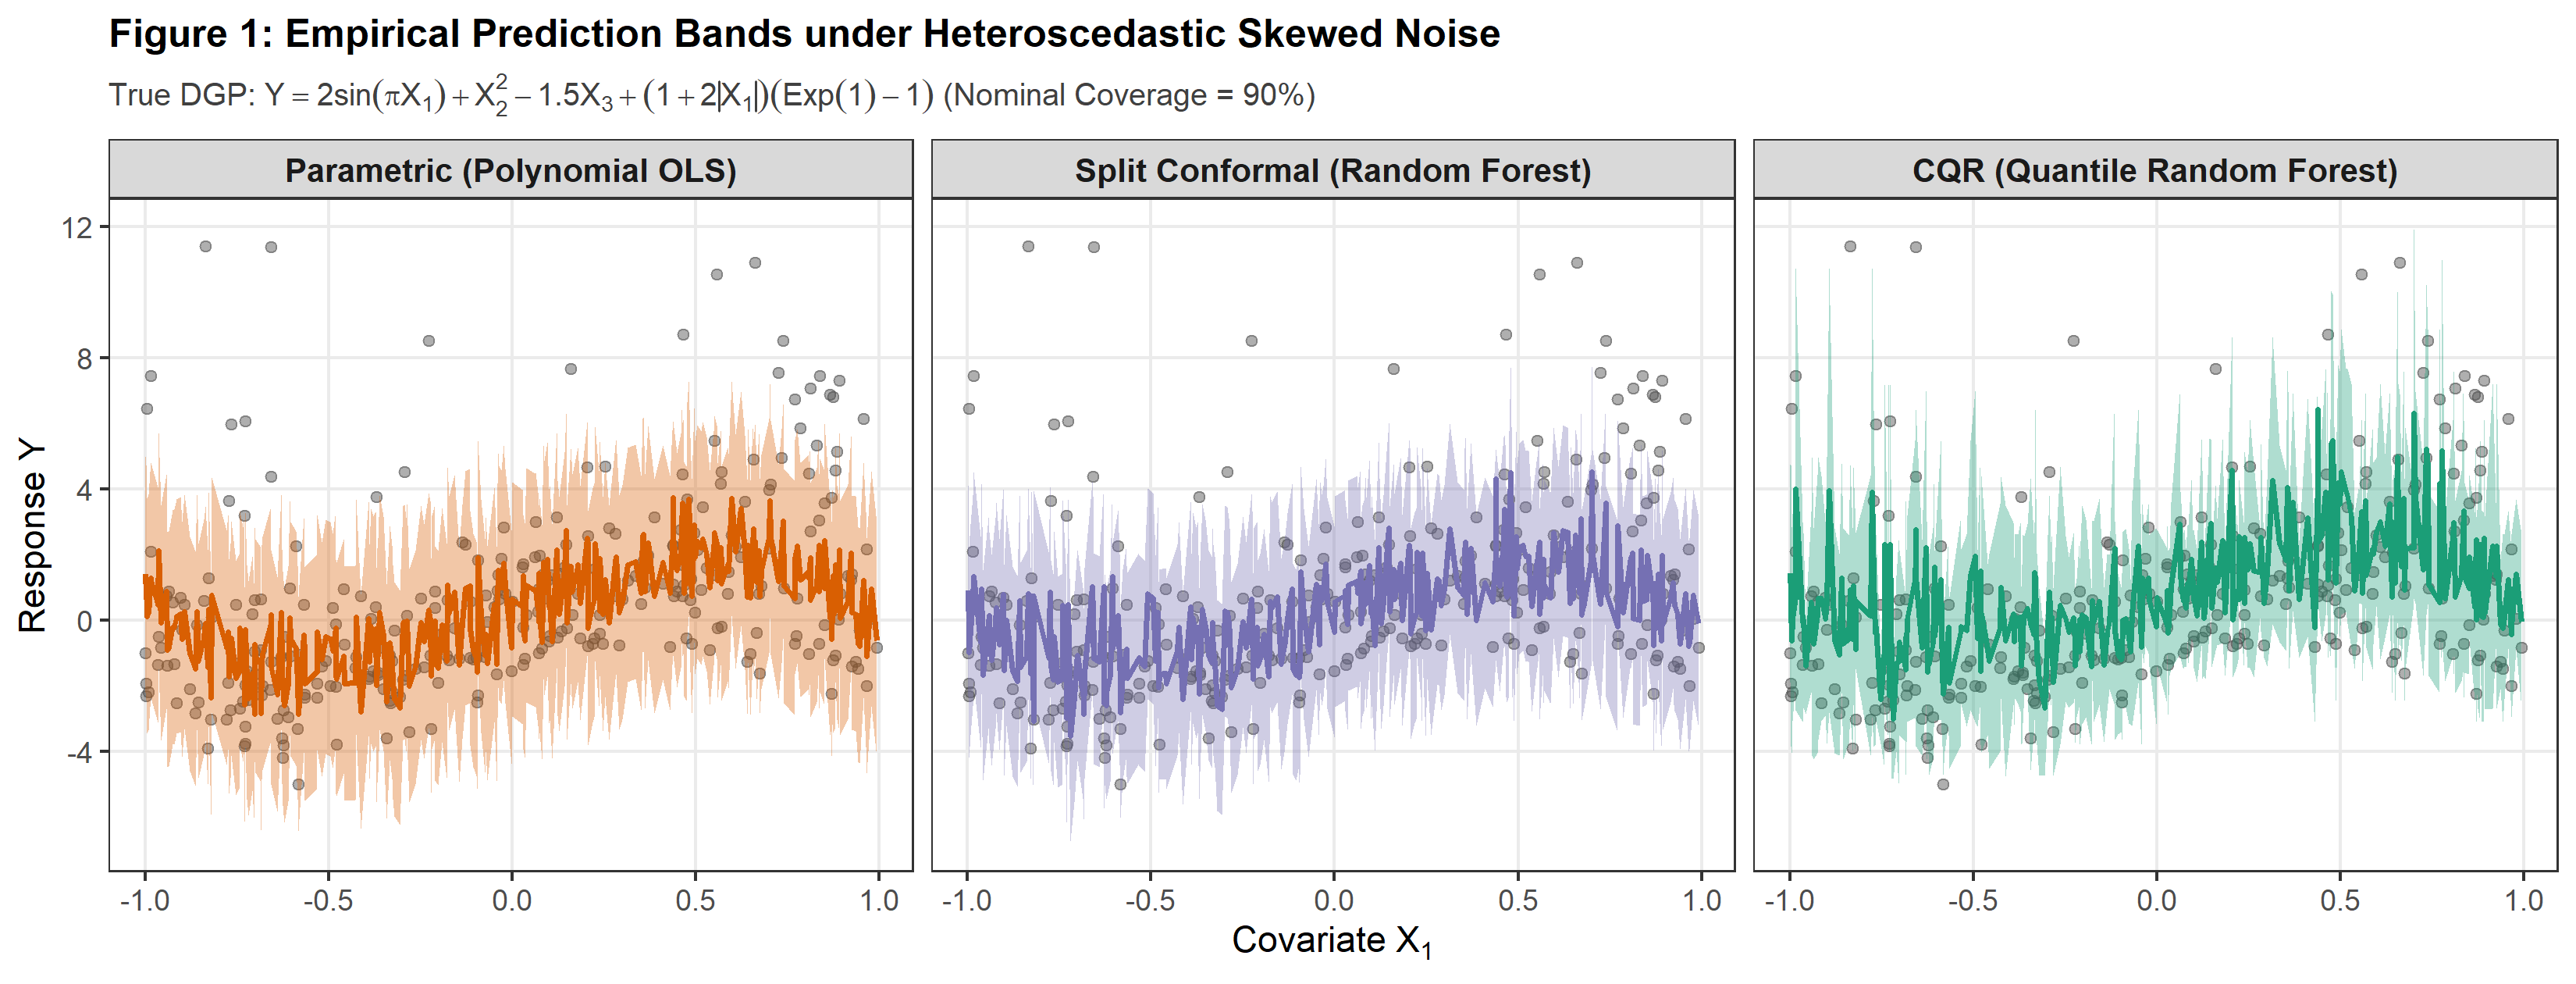
\includegraphics[width=0.95\textwidth]{fig1_prediction_bands.png}
\caption{Empirical $90\%$ prediction bands along feature $X_1 \in [-1, 1]$ under Regime III (heteroscedastic skewed noise) for Parametric OLS (left), Split Conformal RF (center), and CQR (right). Note how CQR narrows near $X_1 = 0$ and broadens as $|X_1| \to 1$ while matching noise skewness.}
\label{fig:bands}
\end{figure*}

Figure~\ref{fig:bands} illustrates the $90\%$ prediction bands along feature $X_1 \in [-1, 1]$ under Regime III:
\begin{itemize}
    \item \textbf{Parametric Polynomial OLS (Left Panel):} Generates a rigid band of nearly constant width. Because it cannot adjust to the local noise $\sigma(X_1) = 1 + 2|X_1|$, it over-covers near $X_1 = 0$ (where noise is small) and under-covers near $|X_1| = 1$ (where noise is large).
    \item \textbf{Split Conformal Random Forest (Center Panel):} Captures the non-linear mean curve $\mu(X_1)$. However, because its non-conformity score is based on unweighted absolute residuals $|Y - \hat{\mu}(X)|$, the resulting interval width $2\hat{q}_{1-\alpha}$ remains globally constant across $X_1$.
    \item \textbf{Conformalized Quantile Regression (Right Panel):} Produces an adaptive envelope that narrows to width $\approx 3.2$ near $X_1 = 0$ and widens to $\approx 10.5$ at $|X_1| = 1$. It also accommodates the positive skewness of $\text{Exp}(1) - 1$, extending further above the predicted curve than below it.
\end{itemize}

\begin{figure*}[!t]
\centering
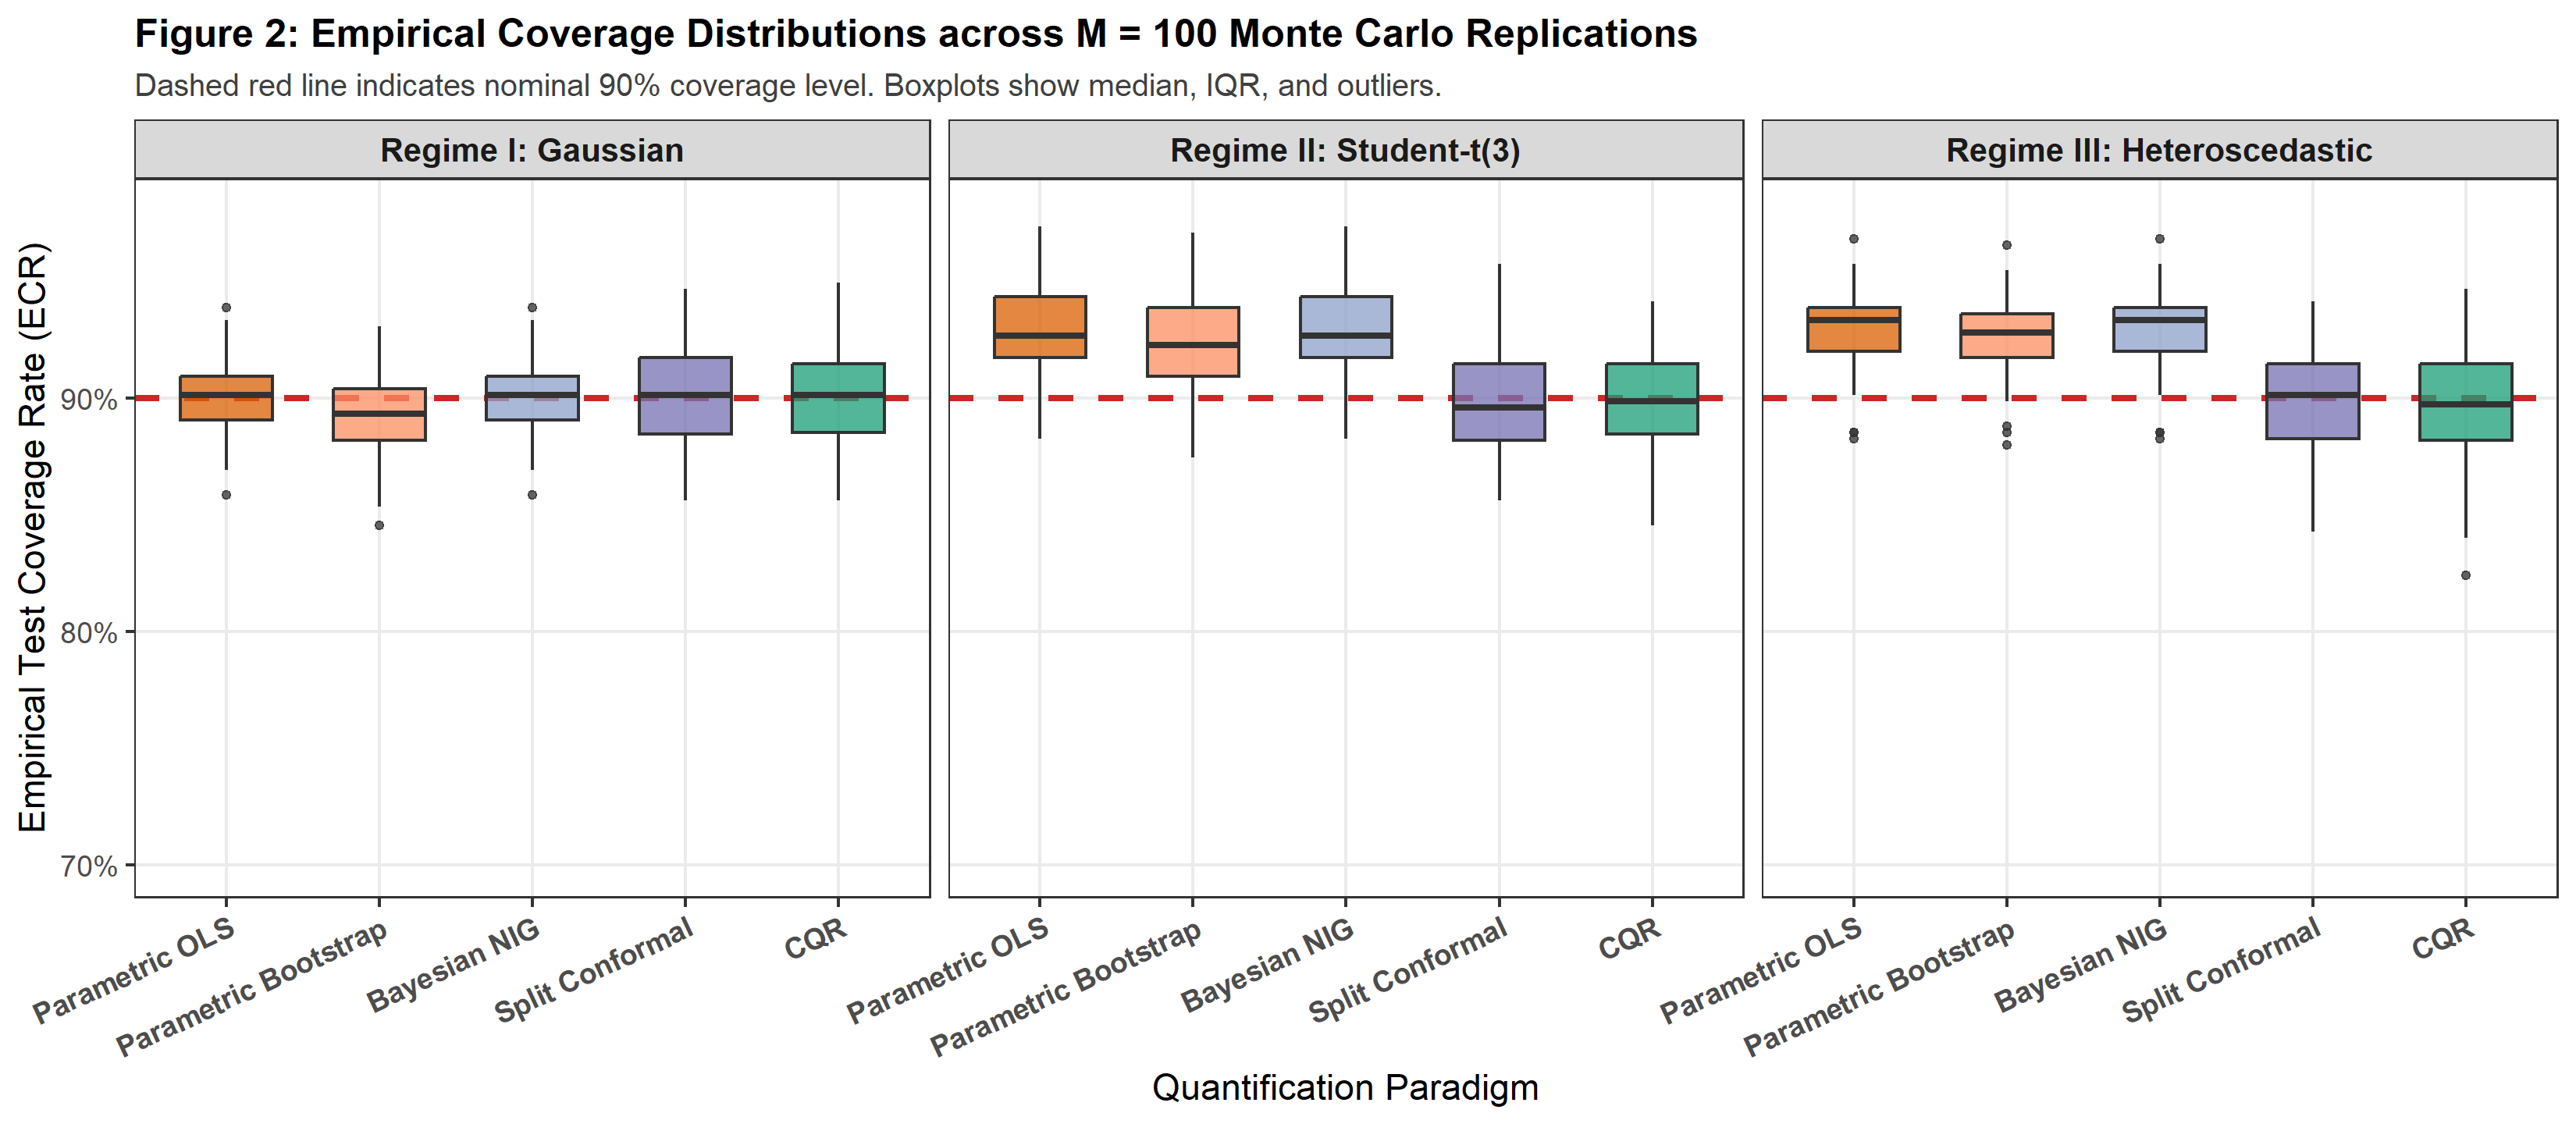
\includegraphics[width=0.92\textwidth]{fig2_coverage_distribution.png}
\caption{Empirical coverage distributions across $M = 100$ Monte Carlo replications relative to the nominal $90\%$ reference line across Regimes I, II, and III. Conformal methods maintain exact marginal coverage across all three regimes.}
\label{fig:coverage}
\end{figure*}

Figure~\ref{fig:coverage} shows boxplots of empirical coverage rates across the $M = 100$ Monte Carlo replications relative to the nominal $90\%$ reference line:
\begin{itemize}
    \item In \textbf{Regime I (Gaussian)}, all methods center close to the $90\%$ line. Parametric models show slightly lower dispersion because their likelihood assumptions match the true data-generating process.
    \item In \textbf{Regime II (Student-$t$)} and \textbf{Regime III (Heteroscedastic)}, the boxplots for Parametric OLS, Parametric Bootstrap, and Bayesian NIG shift upward to $92.6\% - 93.0\%$, showing systematic over-coverage.
    \item In contrast, \textbf{Split Conformal} and \textbf{CQR} remain tightly centered on the $90.0\%$ line across all regimes, confirming their distribution-free finite-sample guarantees.
\end{itemize}

\begin{figure*}[!t]
\centering
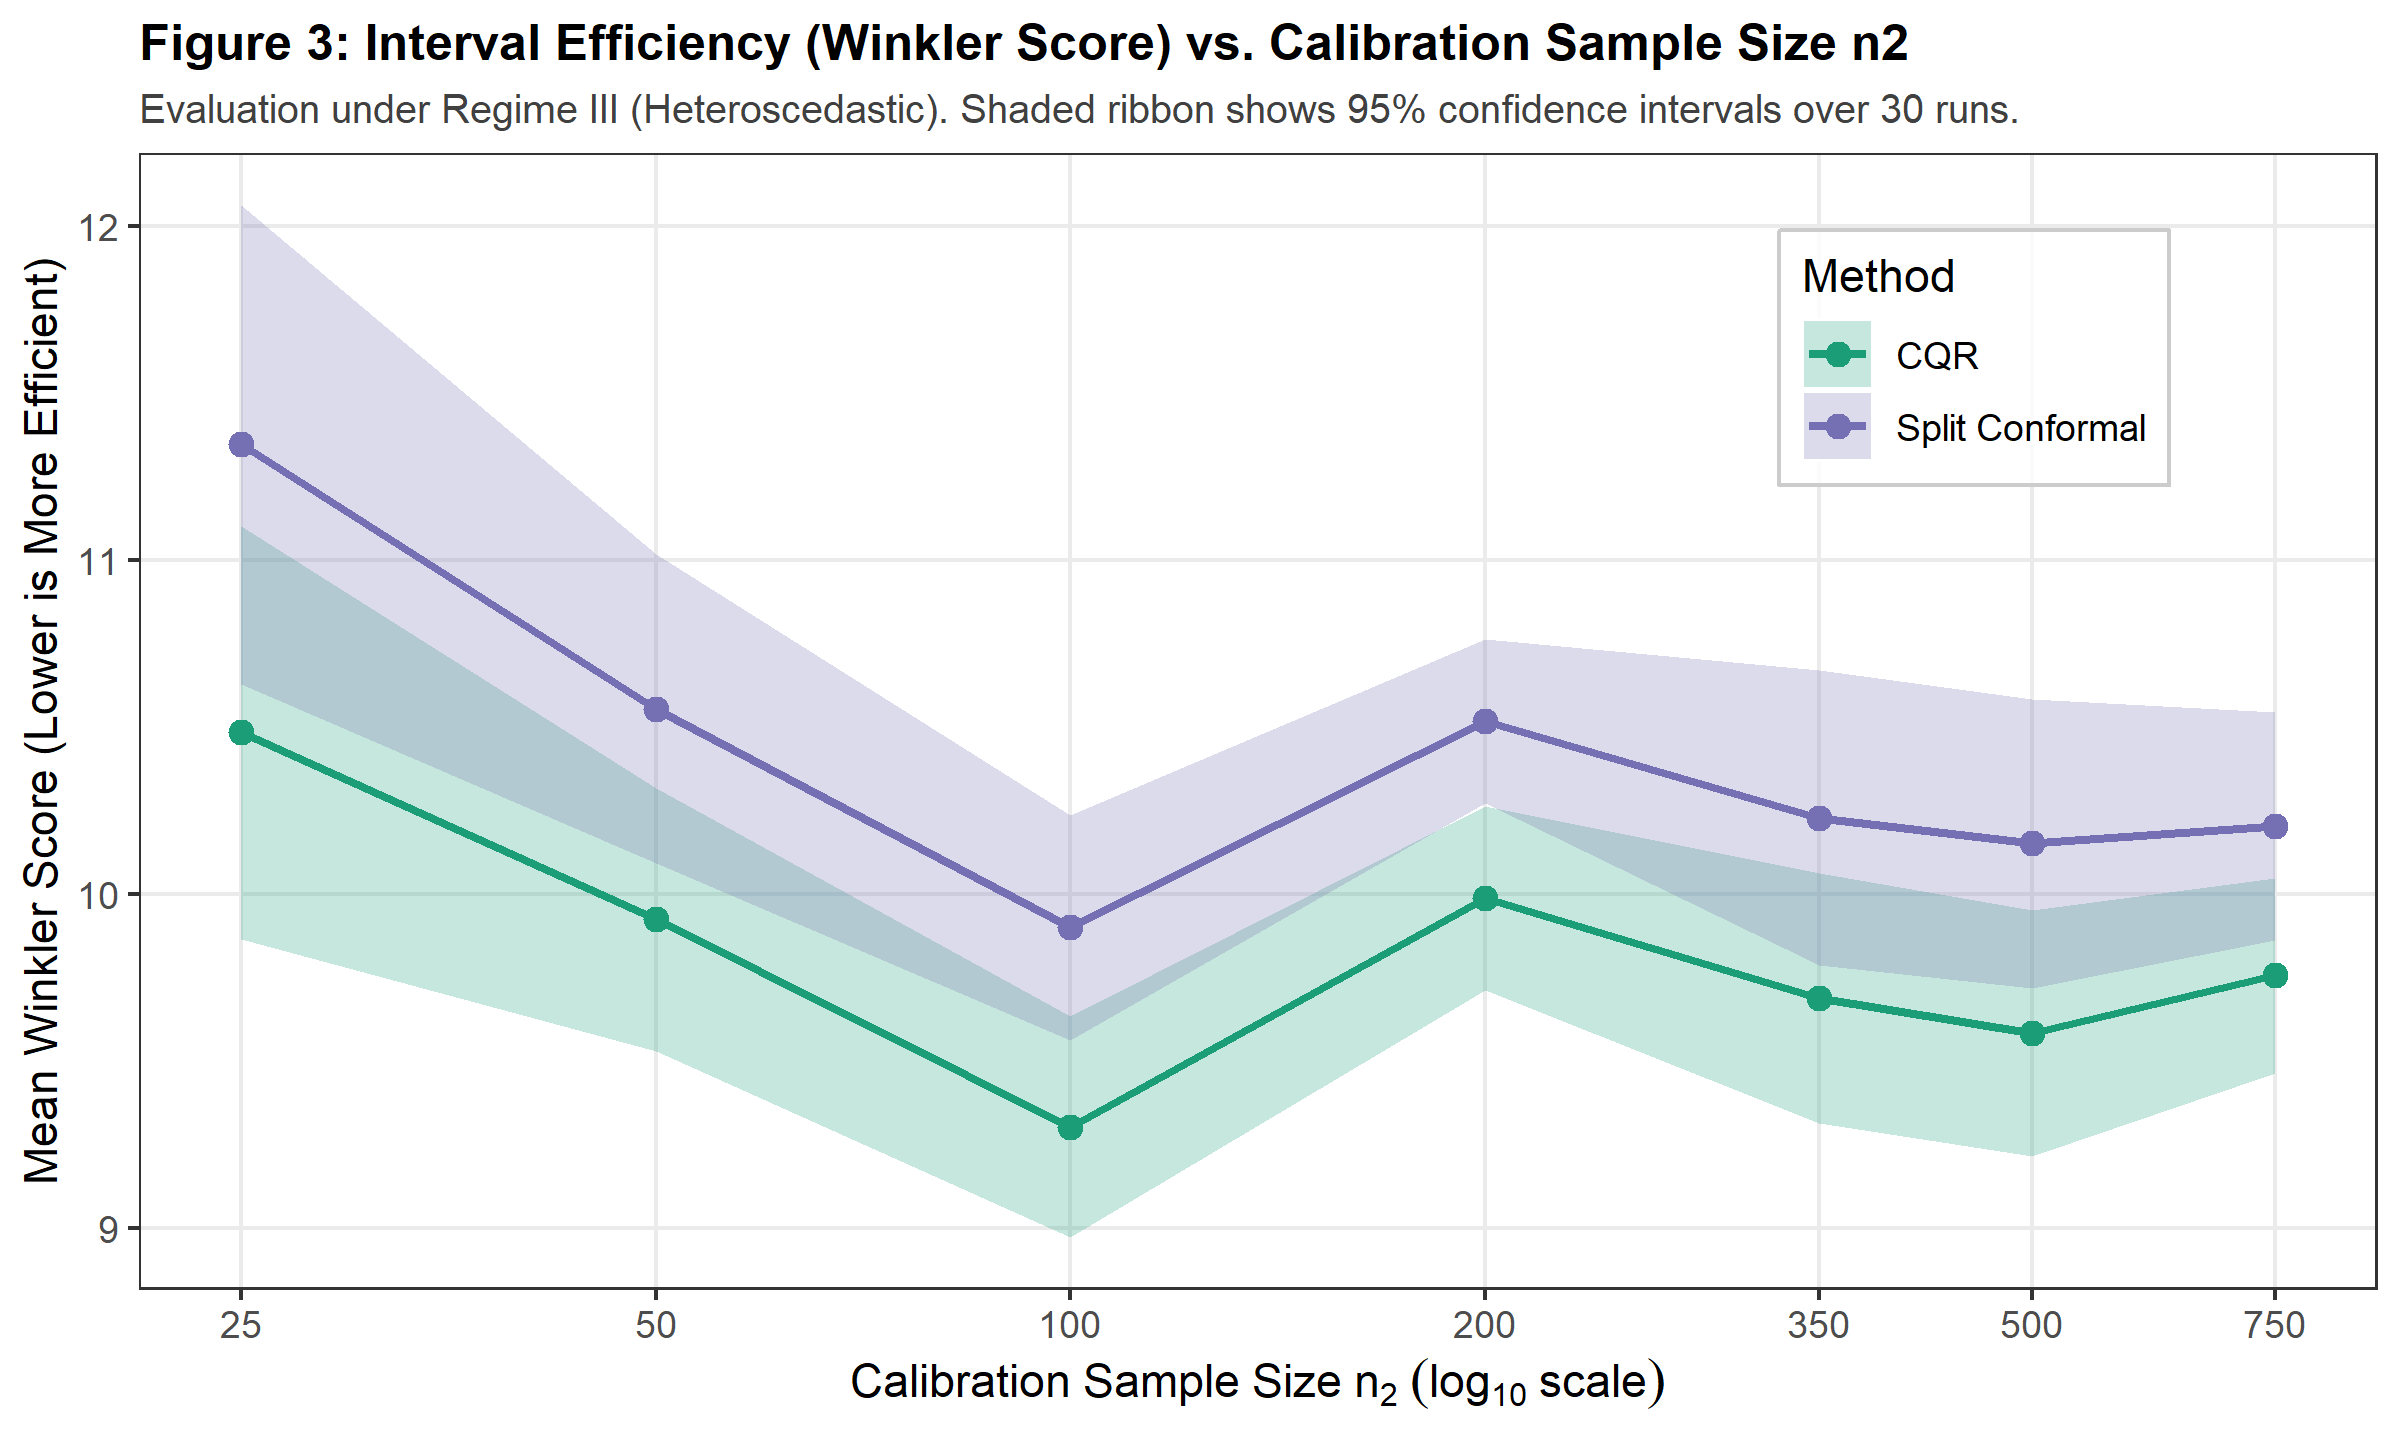
\includegraphics[width=0.75\textwidth]{fig3_winkler_calibration_curve.png}
\caption{Mean interval efficiency (Winkler Score $\pm 1.96 \times \text{SE}$) versus calibration sample size $n_2 \in [25, 750]$ under Regime III. Beyond $n_2 = 200$, calibration variance stabilizes.}
\label{fig:winkler}
\end{figure*}

Figure~\ref{fig:winkler} displays the mean Winkler score ($\pm 1.96 \times \text{SE}$) across calibration sample sizes $n_2 \in [25, 750]$ under Regime III:
\begin{itemize}
    \item When calibration sets are small ($n_2 < 100$), sampling variability in the empirical quantile increases the Winkler score.
    \item As $n_2$ increases beyond $200$, the conformal quantile stabilizes.
    \item Across all calibration budgets, CQR maintains lower Winkler scores than standard Split Conformal, highlighting the efficiency gain from adaptive quantile modeling.
\end{itemize}

\section{Theoretical Discussion \& Practical Considerations}\label{sec:discussion}

\subsection{Sample-Splitting Trade-off ($n_1$ versus $n_2$)}
Split conformal prediction requires partitioning $N$ observations into $n_1$ training points and $n_2$ calibration points, leading to a practical trade-off:
\begin{enumerate}
    \item \textbf{Under-allocating to Training ($n_1 \ll N$):} Increases the base model's estimation error. For a $\beta$-smooth regression function in $d$ dimensions, estimation error scales as $\mathcal{O}(n_1^{-2\beta / (2\beta + d)})$. Poorer base predictions result in larger residuals, which in turn leads to wider prediction intervals.
    \item \textbf{Under-allocating to Calibration ($n_2 \ll N$):} Increases the variance of the empirical quantile:
    \begin{equation}
    \text{Var}(\hat{q}_{1-\alpha} \mid \mathcal{D}_1) \approx \frac{\alpha(1 - \alpha)}{n_2 \, [f_R(q_{1-\alpha})]^2}.
    \end{equation}
    This causes conditional test coverage $\mathbb{P}(Y_{n+1} \in \hat{C}_n(X_{n+1}) \mid \mathcal{D}_n)$ to fluctuate around the marginal $1 - \alpha$ target. Vovk~\cite{vovk2012} showed that the conditional coverage variance scales as $\mathcal{O}(1/n_2)$.
\end{enumerate}

When total sample size is small ($N < 300$), CV+ or Jackknife+ (Barber et al.~\cite{barber2021}) should be preferred to avoid splitting data. When $N$ is moderately large, allocating $65\% - 75\%$ of the non-test data to training ($n_1$) and $25\% - 35\%$ to calibration ($n_2$) provides an effective balance.

\subsection{Marginal versus Conditional Coverage Limits}
Conformal prediction guarantees valid marginal coverage:
\begin{equation}
\mathbb{P}\big(Y_{n+1} \in \hat{C}_n(X_{n+1})\big) \ge 1 - \alpha.
\end{equation}
However, obtaining exact conditional coverage for all feature values $x$:
\begin{equation}
\mathbb{P}\big(Y_{n+1} \in \hat{C}_n(X_{n+1}) \mid X_{n+1} = x\big) = 1 - \alpha \quad \text{almost surely}
\end{equation}
is mathematically impossible for continuous non-atomic distributions in finite samples without producing infinitely wide intervals:

\begin{theorem}[Impossibility of Conditional Coverage; Vovk~\cite{vovk2012}; Barber et al.~\cite{barber2021}]\label{thm:impossibility}
Let $\mathcal{P}$ be the family of all non-atomic distributions on $\mathcal{X} \times \mathbb{R}$. If a prediction interval $\hat{C}_n$ satisfies:
\begin{equation}
\mathbb{P}_{(X, Y) \sim P}\big(Y_{n+1} \in \hat{C}_n(X_{n+1}) \mid X_{n+1} = x\big) \ge 1 - \alpha,
\end{equation}
for almost all $x$ and all $P \in \mathcal{P}$, then for any $P \in \mathcal{P}$ and almost all $x \in \mathcal{X}$:
\begin{equation}
\text{Lebesgue}\big(\hat{C}_n(x)\big) = \infty \quad \text{almost surely.}
\end{equation}
\end{theorem}

CQR resolves this limitation practically: it provides guaranteed marginal coverage under exchangeability, while adapting interval width to local noise levels. If the base quantile models are consistent for the true conditional quantiles (Meinshausen~\cite{meinshausen2006}), CQR asymptotically recovers conditional coverage as sample size grows.

\subsection{Covariate Shift \& Weighted Conformal Prediction}
Theorem~\ref{thm:coverage} requires exchangeability of the observations $(Z_1, \dots, Z_{n+1})$. This condition can fail in practical scenarios:
\begin{enumerate}
    \item \textbf{Time-Series and Serial Correlation:} When observations exhibit autocorrelation ($\text{Cov}(Y_t, Y_{t-k}) \ne 0$), permutation invariance fails. Methods like Adaptive Conformal Inference (Gibbs and Cand\`{e}s~\cite{gibbs2021}) dynamically adjust the nominal level $\alpha_t$ to maintain long-term coverage under distribution drift.
    \item \textbf{Covariate Shift:} Covariate shift occurs when the input distribution changes between training and testing, but the conditional relationship $Y \mid X$ remains unchanged:
    \begin{equation}
    P_{\text{train}}(X) \ne P_{\text{test}}(X), \quad P_{\text{train}}(Y \mid X) = P_{\text{test}}(Y \mid X).
    \end{equation}
\end{enumerate}

Tibshirani et al.~\cite{tibshirani2019} proved that \textbf{Weighted Conformal Prediction} restores exact finite-sample coverage under covariate shift if the likelihood ratio $w(x) = \frac{dP_{\text{test}}(x)}{dP_{\text{train}}(x)}$ is known exactly. The normalized weights are:
\begin{align}
p_i(X_{n+1}) &= \frac{w(X_i)}{\sum_{j=1}^{n_2} w(X_j) + w(X_{n+1})}, \quad i \in \{1, \dots, n_2\}, \\
p_{n+1}(X_{n+1}) &= \frac{w(X_{n+1})}{\sum_{j=1}^{n_2} w(X_j) + w(X_{n+1})}.
\end{align}
When the density ratio $w(x)$ is estimated from data (e.g., using logistic regression or density estimation), the exact guarantee is relaxed to an asymptotic bound governed by the estimation error $\|\hat{w} - w\|$.

\subsection{Methodological Considerations \& Limitations}
Our empirical findings should be considered alongside several practical factors:
\begin{enumerate}
    \item \textbf{Simulation Replication Budget:} While $M = 100$ Monte Carlo replications provided sufficient power to distinguish coverage differences under misspecification ($p < 10^{-15}$), running larger replication budgets ($M \ge 1,000$) would further narrow Monte Carlo standard errors.
    \item \textbf{Data Splitting Overhead:} Split conformal methods require holding out calibration data, reducing the sample size available for training the underlying regression model.
    \item \textbf{Repeated Split Correlation:} Repeated random splits of the Boston Housing dataset share observations, meaning performance metrics across splits are positively correlated. Therefore, statistics from repeated splits should be interpreted as measures of split stability rather than independent hypothesis tests.
\end{enumerate}

\section{Conclusion}\label{sec:conclusion}
In this paper, we presented a comprehensive theoretical and empirical comparison of five uncertainty quantification methods in machine learning: parametric OLS, the parametric bootstrap, Bayesian Normal-Inverse-Gamma inference, Split Conformal Prediction, and Conformalized Quantile Regression (CQR). 

Our simulation results in R demonstrate that while classical parametric and Bayesian methods achieve optimal interval width under standard Gaussian homoscedastic conditions, they suffer from significant coverage inflation ($92.7\%$ to $93.0\%$ at nominal $90\%$) when error distributions have heavy tails or heteroscedastic noise. In contrast, split conformal prediction and CQR maintain empirical coverage consistent with the nominal $90\%$ target across all tested noise regimes, backed by finite-sample distribution-free guarantees under exchangeability. Furthermore, Conformalized Quantile Regression adapts interval width locally to conditional variance, achieving substantially lower Winkler scores under heteroscedasticity. Conformal prediction provides a practical, mathematically sound approach to uncertainty quantification in modern machine learning.

\bibliographystyle{IEEEtran}
\bibliography{references}

\end{document}
